\documentclass[12pt]{article}
\usepackage[utf8]{inputenc}
\usepackage[norsk, english]{babel}
\usepackage{cite}
\usepackage{hyperref}
\usepackage{color}
\usepackage{rotating}
\usepackage{adjustbox}
\usepackage{caption}
\usepackage{xcolor}

\linespread{1.3}
\newcommand\todo[1]{\textcolor{red}{#1}}
\newcommand{\HRule}{\rule{\linewidth}{0.5mm}}
\setcounter{tocdepth}{5}

\begin{document}
\title{A Review of the Agile Retropsective}

\author{Alf Magnus Stålesen, Bjørn Dølvik}
\begin{titlepage}
\begin{center}

\textsc{\LARGE Norwegian University of Science and Technology}\\[1.5cm]

\textsc{\Large }\\[0.5cm]

% Title
\HRule \\[0.4cm]
{ \huge \bfseries Strengths and Weaknesses of the Agile Retrospective\\[0.4cm] }

\HRule \\[1.5cm]

{\large Authors:}\\

Alf \textsc{Magnus Stålesen}\\
Bjørn \textsc{Dølvik}\\[1.0cm]

{\large Supervisor:}\\

Torgeir \textsc{Dingsøyr}\\[1.0cm]

{\large \today}

\end{center}
\end{titlepage}

\begin{abstract}
\end{abstract}
\clearpage

\tableofcontents
\clearpage

\part{Introduction}
\section{Background}
Over time the agile retrospective has a tendency to become more repeating and less engaging for the participants in an development project. This can result in the retrospective loosing its value as a place for improvement. 
\todo{Write more here}
\section{Theory}
\section{Terminology}

\section{Thesis}
\todo{To be changed to fit results better}
Through this article we are going to review the agile retrospective practices employed today. Using a ``grounded-theory'' inspired process we will go through existing literature finding strengths and weaknesses of the retrospective. Our goal is to provide a clear overview over the domain and identify, if any, gaps in the current research. 

\clearpage

\part{Method}

\section{Data Collection and searching strategy}
Basing this article on systematic review our data collection is done through several stages: Searching for articles through well acknowledged sources, excluding irrelevant hits and assessing the remainder. Each stage will be described in detail in the following subsections.

\subsection{Semantic Searching}
Before searching the authors decided between them a set of keywords which were to be used as the searching word. The selection of words was aimed towards the agile retrospective, but as the name of this practice has changed over the years we also included Post Mortem. Trying to get a bigger set of data we also included general keywords from the field such as agile practices as articles can be poorly named or described, but still be relevant for this study. With these thoughts in mind we ended up with a set of relevant keywords as can be seen in \autoref{table:keywords}.

\begin{table}[!h]
	\begin{center}
		\caption{Keywords used in searching databases}
		\label{table:keywords}
		\begin{tabular}{ l }
			Keywords: \\ \hline
			Agile Practices \\
			Retrospective \\
			Post Mortem \\
			Software Development \\
		\end{tabular}
	\end{center}
\end{table}

When the list of keywords were complete the selection of databases were decided upon. The criteria for the databases were based upon trying to get a wide span of hits going. This resulted in 2 databases used, Web of science and Scopus, These databases were selected as they had plentiful of search options and between them covered a wide set of journals, see \autoref{table:tools}. 

\begin{table}[!h]
	\begin{center}
		\caption{The databases used for data gathering and some well know}
		\label{table:tools}
		\begin{tabular}{ l | p{0.75\textwidth}}
			Databases: & Journals: \\ \hline
			Webofscience & Information and Software Technology \\ 
			& Software Quality Journal \\
			& International Journal of Information Technology \& Decision making \\
			& ++1400 more \\
			\hline
			Scopus & Information and Software Technology \\ 
			& IEEE Software\\
			& Journal of Systems and Software \\
			& ++5000 others \\
		\end{tabular}
	\end{center}
\end{table}
			
Having selected the set of keywords and tools to use the searching began. Using the boolean operators of AND and OR one search was conducted using each tool. The search string given was the following: 
\begin{center}
	\emph{"Retrospective AND software development OR post mortem AND software development OR agile practices AND software development"}
\end{center}
This search resulted in 1,754 papers that could be relevant for our research.

\subsection{Excluding irrelevant articles}
Excluding articles not relevant for our research became the next step in obtaining data for this literature review. The criteria for exclusion can be found in \autoref{table:datacriteria}. \\

\begin{table}[h!]
	\begin{center}
		\caption{Exclusion criteria for articles}
		\label{table:datacriteria}
		\begin{tabular}{l p{0.75\textwidth}}
		 	\multicolumn{2}{l}{Exclusion criteria}\\
		 	\hline
			1. & Exclude if the article have research domain other than computer science. \\
			2. & Exclude if the article isn't an empirical study. Lessons learned articles and books are in many cases not peer reviewed and we dismiss this as we wish this article to be based on high quality research. \\
			3. & Exclude if the article clearly isn't within the research area of this article. This paper has focus on the software development processes and all articles focusing on technical aspects of software engineering or is in other research area than software development are not relevant. \\
			4. & Exclude article if the focus isn't practices used in software development. \\
		\end{tabular}
	\end{center}
\end{table}

\paragraph{Step 1}
Starting with 1,754 papers the first step was to apply automatic filtering on research area given by the databases. The area we selected was computer science as all other areas are not relevant for this paper. The result of this filtering left us with 801 articles too continue with. 

\paragraph{Step 2}
The next step in the filtering process was to exclude all papers not being peer-reviewed articles. This was also done by the databases automatic filtering. The article types we excluded were books and reviews. This resulted in 266 articles left. 

\paragraph{Step 3}
Having obtained 266 articles of potential relevance for this review, excluding articles not fitting our needs became the next step. First we excluded based on title. If the title clearly described the article as not focusing on the development practices it were excluded, i.e. if an article clearly focused on a technical aspect of some computer system it were excluded. This resulted in 119 articles left in our data collection. 

\paragraph{Step 4}
Left with 119 articles standing we started reading through the abstracts to excluding articles not focusing on the practices used in agile development. The focus of this paper is to bring a better overview of the agile retrospective and papers that focuses on the implementation of agile development or agile development as a part of a project become irrelevant. In the cases were the authors were uncertain about a papers focus, we discussed what potential parts could be relevant and if this didn't give us a result we quickly skimmed the article and looked for potential relevance. If not relevance were found we dismissed the article. This resulted in 48 articles that could be deemed relevant. 

Finally the filtering resulted in 48 peer-reviewed articles that were relevant to our research area of agile retrospectives. 

\subsection{Article selection}
These 48 peer-reviewed articles were of varying degrees of relevance for our study. We wanted to limit our final articles to the most relevant pieces. In order to do this final selection we constructed a grading scheme based on the focus of the articles, where a high grade meant a high focus on retrospectives or post-mortems. 

\begin{table}[!h]
	\centering
	\caption{Grading scheme for article selection}
	\label{table:article_grading}
	\begin{tabular}{l | p{0.5\textwidth}}
		\hline
		Grade & Criteria \\
		\hline
		1-3 & Mentions retrospectives , but does not discuss in depth \\
		4-7 & Mentions and discusses retrospectives  or discusses relevant practices, activities. \\
		8-10 & Focus on retrospectives or the practices relevant to a retrospective. \\
	\end{tabular}
\end{table}		

Once the grading scheme was agreed upon both group members read through all the articles separately, grading the articles. The grading were written into a document and the average was considered the final score. The abstract of the article was read, in order to understand the whole content and intent of the article. The grading was very similar with few outliers. Any outliers were re-read and discussed together and if necessary. Once the final score was set any articles with a score of less than 7 were eliminated. The grade of 7 was chosen we deemed everything below not sufficiently relevant. Eliminating the low graded articles resulted in a set of articles who either focused on retrospectives or contained a high level of relevant discussion. This resulted in 19 articles that were considered relevant enough. This was considered a satisfactory amount of articles. Thus the article search ended.


\clearpage

\part{Results}
The results from our literature review presented us with two primary views on how to evaluate the agile retrospective practices. The first one being the practices used when conducting an agile retrospective. The second one regards enthusiasm for the agile retrospective. Through this part we will present our findings on these two views, but first we will give an overview of the studies used in this literature review. 

\section{Overview of Studies}
In \autoref{table:studies-research-methods} we provide an overview of what kind of research methods is used in the different studies. 53\% of the research material we have used is purely empirical research. This research consists of single-case studies, multiple-case studies, experiments and literature reviews. This material we will draw our conclusions upon 

The remaining 47\% of the research material consists of experience reports and methodology suggestions. We recognize that experience reports are not empirical studies, but we believe they will help provide a broader understanding of the research area, as Wang et al. ~\cite{Wang2012} states. We will however not draw any definite conclusions based on the experience reports will use them for supporting our own assumptions. The same goes for methodology suggestions. 

\begin{table}[!h]
	\centering
	\caption{Studies by research method}
	\label{table:studies-research-methods}
	\begin{tabular}{ p{0.3\textwidth} p{0.3\textwidth} p{0.3\textwidth}}
		\hline
		Research method & Number & Percent \\ \hline
		Single-case & 2 & 10.5 \\
		Multiple-case & 6 & 31.6 \\
		Experiment & 1 & 5.2 \\
		Experience reports & 6 & 31.6 \\
		Literature review & 1 & 5.2 \\
		Other* & 3 & 15.7 \\
		\\
		Total & 19 & 100 \\ \hline
	\end{tabular}
	*``Other'' refers to methodology suggestions
\end{table}

Looking at \autoref{table:studies-publications} we see the publications channels of the different studies. The biggest distribution channels being Journal articles, with 58\%, and conference papers, with 37\%. The remaining 5\% is consisting of one book as we treat as a methodology suggestion. IEEE and Information and Software Technology is the two journals containing most studies and the different agile 20xx conferences having the most studies for conferences. 

\begin{table}[!h]
	\centering
	\caption{Studies by research method}
	\label{table:studies-publications}
	\begin{tabular}{ p{0.43\textwidth} p{0.15\textwidth} p{0.15\textwidth} p{0.15\textwidth}}
		\hline
		Puplication channel & Type & Number & Percent \\ \hline
		IEEE & Journal & 4 & 21 \\
		Information and Software Technology & Journal & 3 & 16 \\
		Agile 20xx & Conference & 3 & 16 \\
		The Journal of Systems and Software & Journal & 2 & 11 \\
		XP 20xx & Conference & 1 & 5 \\
		IEEE  20xx & Conference & 1 & 5 \\
		Profes 20xx & Conference & 1 & 5 \\
		Empirical Software Engineering & Journal & 1 & 5 \\
		ESERNET & Journal & 1 & 5 \\
		Euromicro & Conference & 1 & 5 \\
		Agile Retrospectives Making Good Teams Great! & Book & 1 & 5 \\
		\\
		Total & & 19 & 100 \\ \hline
	\end{tabular}
\end{table}

\section{Practices of the Agile Retrospective}
One of our main findings reading through the selected article where that there are many ways to conduct a retrospective. Categorizing our findings we ended up with three phases a retrospective contains. These three are: before, during and after the retrospective meeting. We will go through each of these phases presenting our findings.

\section{Before the Retrospective}
In this section we go through the work needed to be perfomed before the retrospective. This is arranged in both practical tasks as well as principles that should be kept in mind in order to hold a successfull retrospective. The tasks discussed are ``Wish to improve'', ``Declaring a goal'', ``Participants'', ``Collect objective data'' and ``Which technique to use''. 

\subsection{Wish to improve}
The retrospective is conducted out on an interestet to improve the processes in an orginization, and deciding to use the retrospective as a tool. Dingsoyr~\cite{Dingsoyr2005} describes the retrospecive as a method for organisational learning. So the holding of a retrospective need to be based on a wish to improve through organisational learning. Especially in software engineering has this attention to knowledge management increased, in the hope of improving processes through learning from the past. The wish to improve should not be limited to just the management, but a culture of knowledge management should also take place in the organization units themself.

\subsection{Declaring a goal}
A retrospective is not a self contained activity, and there are multiple actions that can be taken before and after the actual retrospective in order to ensure a successful. Dingsøyr~\cite{Dingsoyr2005} lays out a set of steps for conducting a postmortem review. The first step is the project head deciding to hold the retrospective, followed by the declaring this intent to the project. Thereafter the participants for the exercise should be selected. Then work to prepare for the retrospective can then begin. It is important that the project participants start understanding and preparing for the intent of the retrospective. The participants need to understand that it is their 

\subsection{Gather Data}
The work done before the retrospective should be focused on gathering objective data, and the relevant context concerning the data. Dingsøyr, Birk and Stålhane~\cite{Moe2001}  describe how one should include both positive and negative data. A retrospective should not be wholly focused on the positive and negative aspects of a project, this should be reflected in the gathering of data. It is also important to be open to collection data and feedback from all possible sources, as this gives a more complete picture of the issues.

\subsubsection{Survey} There are different ways of gathering information. Collier, DeMarco and Fearey~\cite{Collier1996} describes the need for a defined process, suggesting starting with a survey to gather objective information. The survey is chosen because it is possible to be a quick low investment option where the project team's input can be gathered in a wide range of projects. Especially large projects can benefit from electrionic surveys, as it can allow the gathering of large volumes of timely feedback. Surveys also provide anonymity, giving participants more room to be honest. An example survey is provided by Collier et al. in \autoref{figure:survey}.

\begin{figure}[h!]
	\centering
	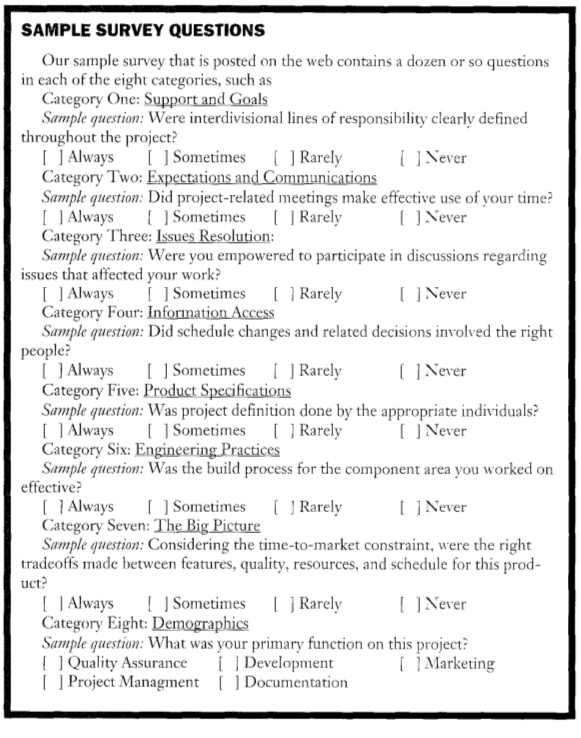
\includegraphics[width=\textwidth]{figures/survey.png}
	\caption{An example survey provided by Collier, DeMarco and Fearey~\cite{Collier1996}}
	\label{figure:survey}
\end{figure}

\subsubsection{Interview} Another option is to interview a sample of the participants or stakeholders in the project. This is a usually a more time intensive method and more resource intensive. Interviews are a very powerful information gathering tool, allowing the interviewee to share data with a personal context and connection. A benefit of interviewing is the possibility of gathering points of view and data from relevant sources who will not attend the actual retrospective. This might include customers, managers or team members with other commitments. Another potential data collection method is monitoring and observing the project as it develops taking time stamped pieces of data for later use, this might for example include copies of email or other communication. 

\subsubsection{Collect objective data} Collier, DeMarco and Feary~\cite{Collier1996} describes the need for objective data to support the decisions of the retrospective. The data collected should when seen in a context provide an outline of actual issues of the project. The data should support the retrospective in identifying the biggest areas that can be improved. In order to maximize the efficency of the retrospective the issues that can be improved should be ordered in a list by the highest return on time invested. The project can then use this as a work plan for its future improvements. The data collection also allows for comparison between previous projects, by having a measuring stick the project can compare itself to external projects. By comparing the current projects to other projects the retrospective can base its decisions on a wide range of data. The hard data that is collected will also help the discussion, and focus it on the issues, as a retrospective led entierly through memory can be biased as described in Bjarnson and Regnell~\cite{Bjarnson2012} Memory bias is the selective nature of human memory, and can forget, ignore or misunderstand events. This memory bias can lead to potential improvements going lost. The objective data should aim to cover the metric types important to supporting retrospective decision making. These metric are cost, schedule and quality.

\begin{table}[!h]
	\centering
	\captionsetup{justification=centering}
	\caption{objective data metrics, with examples}
	\label{table:objective_data_metrics}
	\begin{tabular}{| l | p{0.5\textwidth} |}
		\hline
		Metric type: & Description \\ \hline
		Cost & The actual costs for issues and events during the project phase. This can include but is not limited to development, testing, quality control, customer meetings and internal meetings. \\ \hline
		Schedule & The original schedule compared to the actual performed schedule. Included should be an overview over any missed deadlines. \\ \hline
		Quality & Defects, bugs and problems. As well as their detection rate and fix rate. \\   
		\hline
	\end{tabular}
\end{table}

Through logging observations a team can get a clear picture of the actual events of the project. By making the observations pieces of date-stamped data a project can prepare for an ``Evidence based timeline'' described by Bjarnason and Regnell~\cite{Bjarnason2012}. These observations have to be clear pieces of data that can be interpeted at a meeting, such as reports, graphs, meetling logs and communication logs. If data collected can not be used as an input the future steps of the retrospective the data should be processed into a usable form. 

\subsection{Preparing the Retrospective}
A retrospective should be planned in advance, and should be tailored to the needs and goals of the project. Derby and Larsen~\cite{Derby2007} lists a set of activities that can be used to generate insight and produce valuable evaluation of project. The activity chosen should be suited for the type retrospective, depending on the goal and nature of the exercise. We elaborate on some of the more common activities in \autoref{subsec:which-techniques}. Other factors that should be accounted for is setting the date, providing the physical materials needed and often planning food. The date is especially important as one should accomedate as many possible participants as possible. The physical materials might depend on the activity selected, but typically include markers, post its and paper. The need for food might be different from retrospective to retrospective, but typically the length of a retrospective require some sort of lunch break. In some cases, especially after a release, the food eaten at a retrospective might be part of the reward for finishing the project phase.


\subsection{Participants}
There are multiple concerns on who should be the participants of the retrospective.  The paticipants are the most important part of the retrospective, as their input and reflections results in the output that makes the retrospective valuable. Therefore it is important that the participants feel safe in sharing their toughts and experiences concerning the project. A retrospective should include representatives from all involved units of the development, included but not limited to planning, development and testing. 

The units involved would naturally vary from project to project. Dingsøyr eliminates the managers~\cite{Dingsoyr2005} from participating in the retrospective, as the project members might be intimidated from sharing all their thoughts since the managers are responsible for evaluating employees. In addition stakeholders such as customers being present can shift the topics from the issues that the team can learn from over to customer relations. 

The presence of the customer might make the team reluctant in bringing up bad experiences with the customer's representative, such as bad communication or long response time. 

The facilitator can either be the project manager, or an external facilitator. An external facilitator has the advantage of seeing the project with a fresh set of eyes, and can potentially lead the team to viewing their problems from a different angle. The facilitator should be trained and prepared to hold the retrospective, it is also important that the facilitator inspires trust in the participants, in order to let them share as many viewpoints as possible.

\section{During the Retrospective}
The second phase of a complete agile retrospective is conducting the retrospective meeting. Here our literature review found that several different techniques were used in practices. Following we will describe techniques used and suggested by the research literature.

\subsection{Techniques Identified} \label{subsec:technqiues-identified}
\subsubsection{KJ-sessions}
KJ-sessions are often mentioned in the articles. Dingsøyr, Moe and Nytrø~\cite{Moe2001} describes how they conducted a KJ-session: 
\begin{quote} We used a technique named after a Japanese ethnologist, Jiro Kawakita - called \"the KJ-method\". For each of these sessions, we give the participants a set of post-it notes, and ask them to write one \"issue\" on each. We usually hand out between three and five notes per person, depending on the number of participants. After some minutes, we ask one of them to attach one note to a whiteboard and say why this issue was important. Then the next person would present a note and so on until all the notes are on the whiteboard. The notes are then grouped, and each group is given a new name. 
\end{quote}
This description is very much similar with description given by other researcher with only minor differences. An example of an output from a KJ-session is provided in \autoref{figure:kj-session}. Such as the number of post-it notes varying or instead of giving a fixed number of post-it notes one give the participants a fixed time to finish writing down the issues. Following a KJ-session there are cause analysis sessions, as the KJ-method only identifies the issues rather than analyze them. We describe different cause analysis techniques below. 

\begin{figure}[h!]
	\centering
	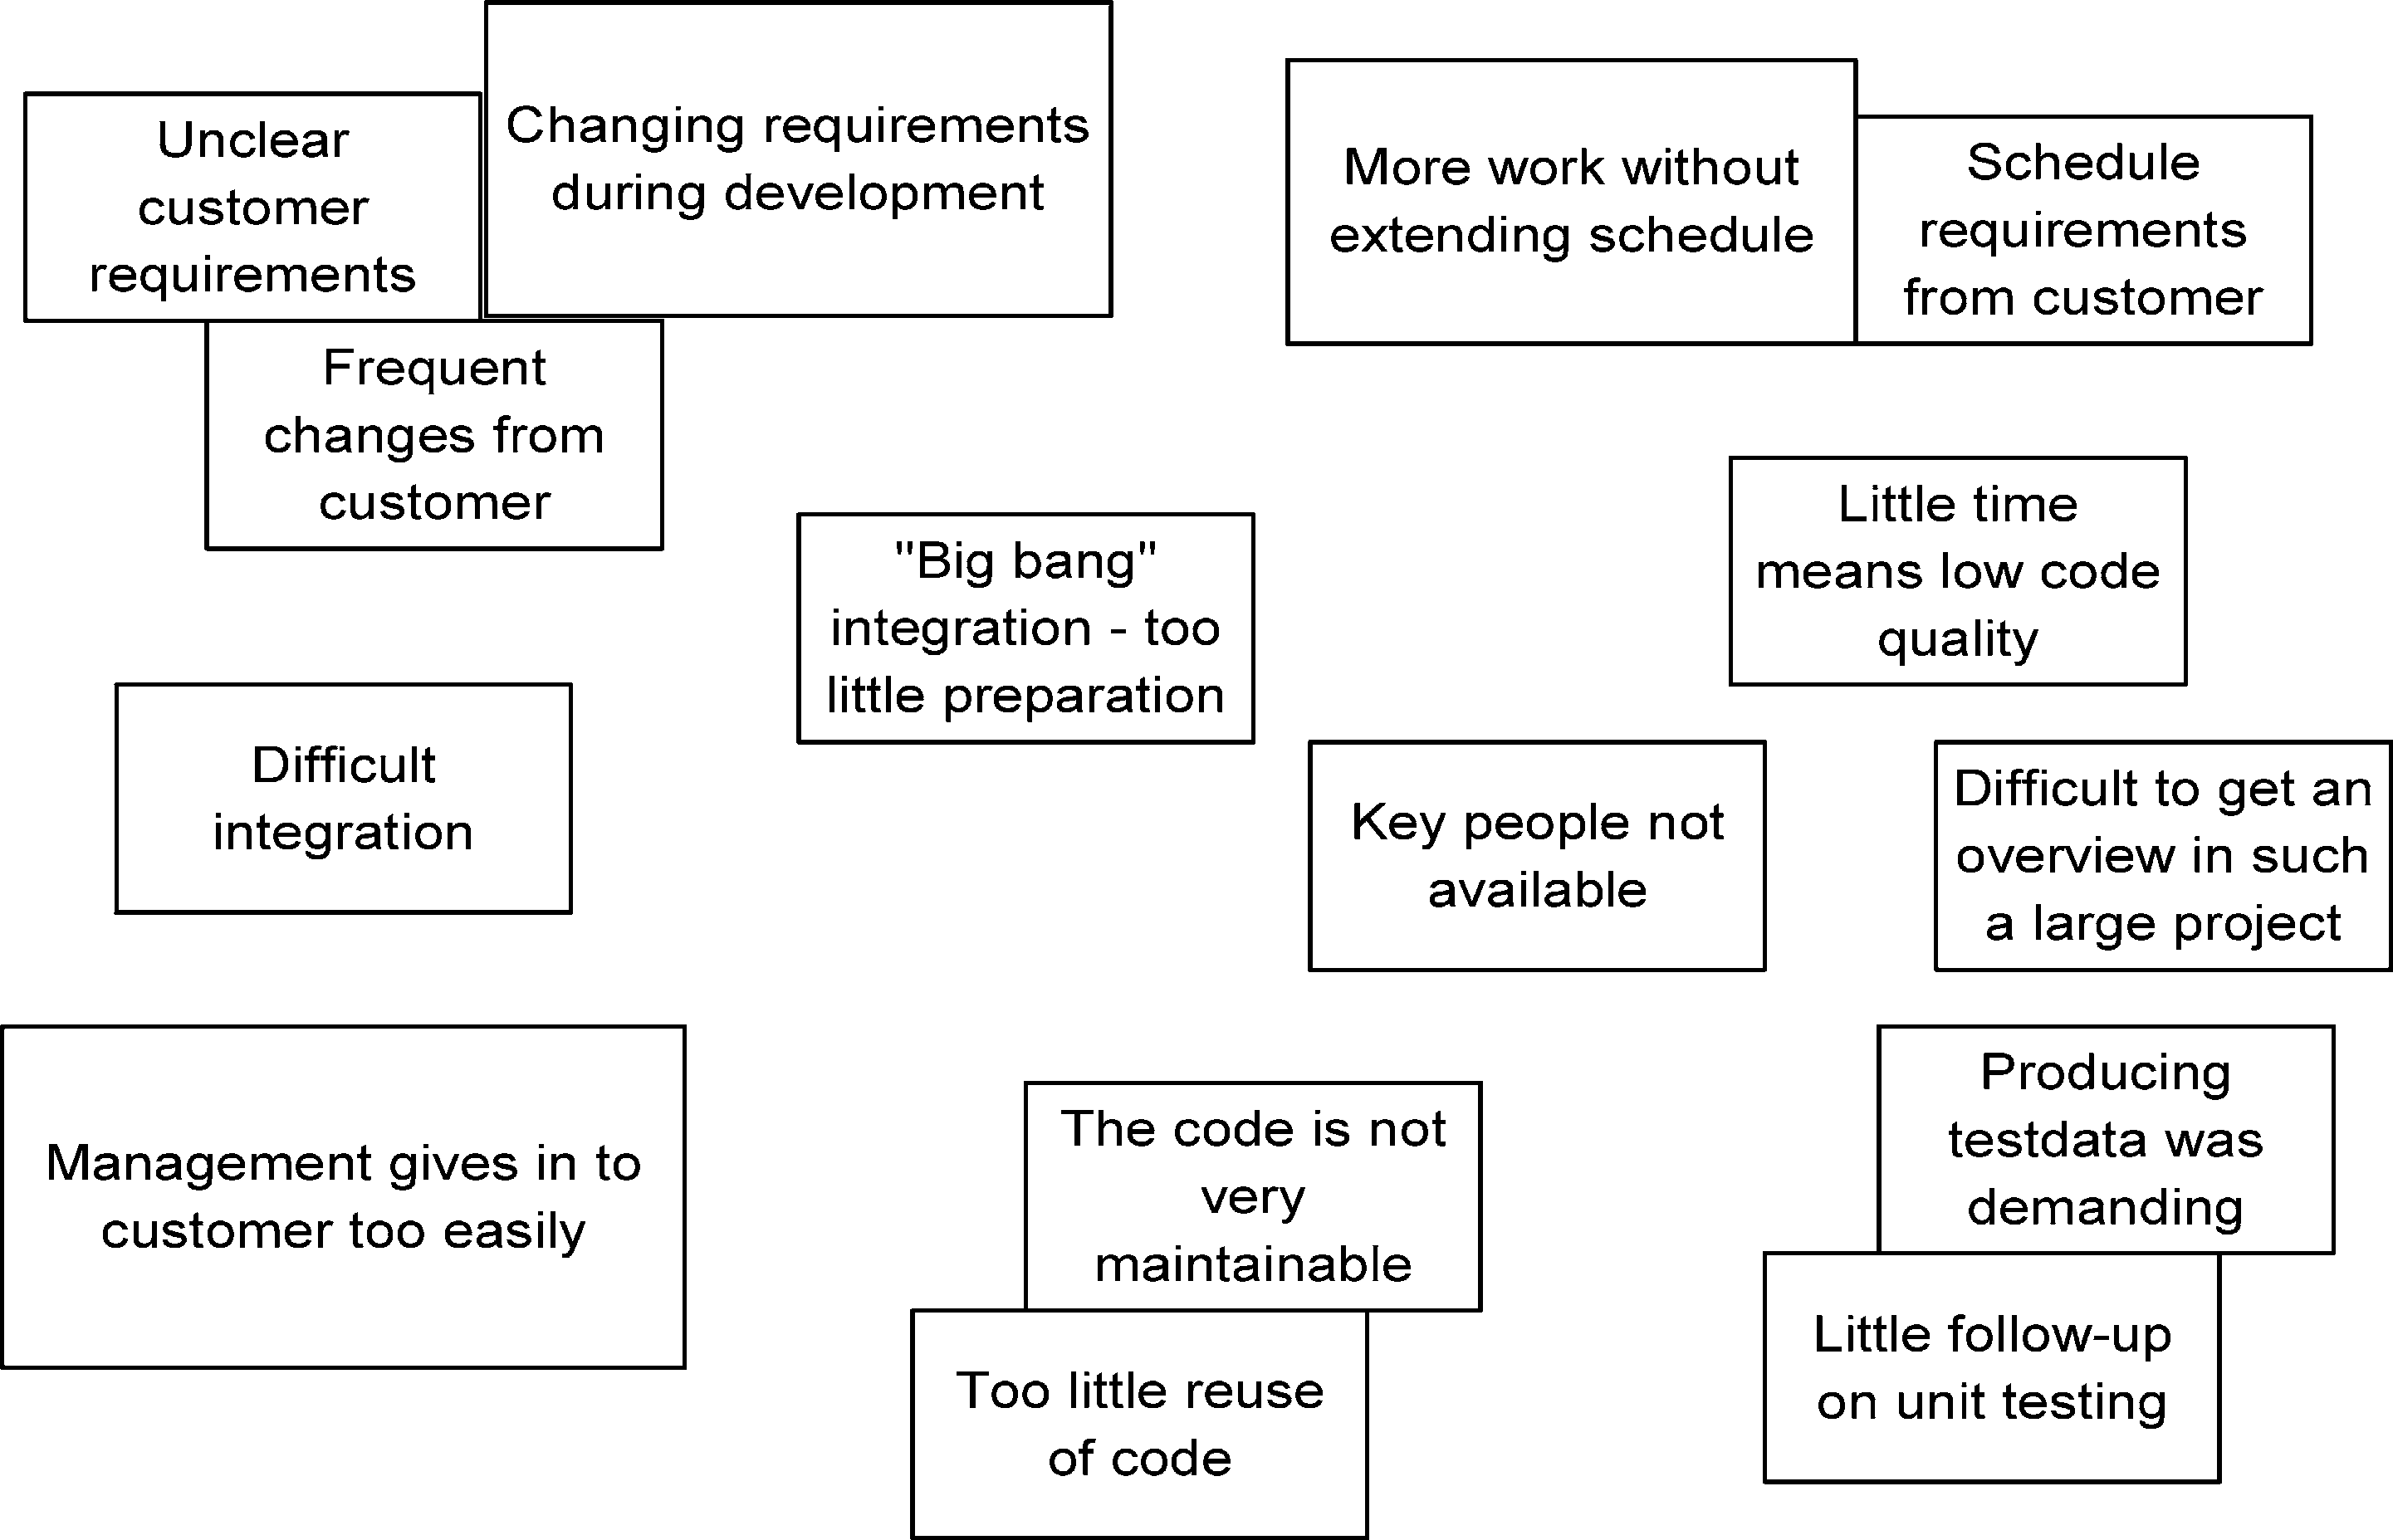
\includegraphics[width=\textwidth]{figures/KJ-session.png}
	\caption{An graphic of the finished board after a KJ-session, provided by Dingsøyr~\cite{Dingsoyr2005}}
	\label{figure:kj-session}
\end{figure}

\subsubsection{Keep, Problem, Try}
Keep, Problem, Try, also known as KPT, is described by Kinoshita~\cite{Kinoshita2008} and works as follows: One split a white board into three areas. One for Keep, one for Problem and one for Try. The session follows with the participants writing down positive feelings on the Keep area of the board, negative feelings on the Problem area. Finally the last area is filled with Try items that one tries to do in the next iteration of the project. This gives the opportunity that the team obtains feedback from oneself, according to Kinoshita. We have provided an example of a KPT board as described by Kinoshite in \autoref{figure:kpt}. 

\begin{figure}[h!]
	\centering
	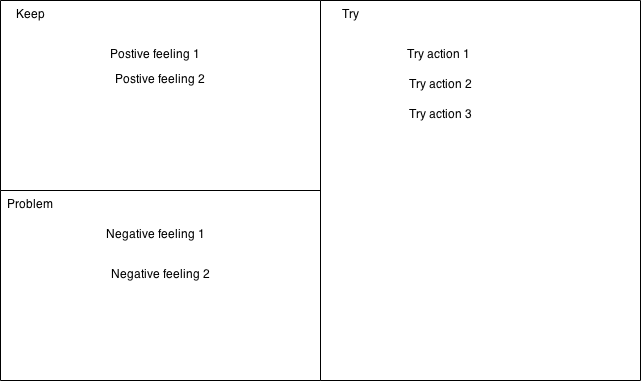
\includegraphics[width=\textwidth]{figures/kpt.png}
	\caption{An example KPT board as described by Kinoshita ~\cite{Kinoshita2008}}
	\label{figure:kpt}
\end{figure}

\subsubsection{Estimation Retrospective}
Estimation Retrospective is another technique mentioned by Kinoshita~\cite{Kinoshita2008}. This technique evaluates the time estimation for the current development iteration. The process is to go through each task and control whether the time estimate is close to actual time used. If there are any differences one discuss possible causes for this. The results are then used when estimating for the next retrospective. Kinoshita described how they used a whiteboard to visualize the estimations; All tasks using the estimated time would be placed in the middle, while those using shorter would be placed to left side and those exceeding the estimation on the right. 

\subsubsection{Experience Reports}

\subsubsection{Positive Strokes}
Positive strokes are a technique used during special events such as releases or exchange of members, according to Kinoshita~\cite{Kinoshita2008}. Its focus is to give each individual member a positive feedback from the rest of development team. They it works is that every member gets a card which they write their name on. The card is then passed around and each member write a positive comment about the owner of the card. The card are then returned to the owner. An example card is provided by Kinoshita in \autoref{figure:positive-strokes}.

\begin{figure}[h!]
	\centering
	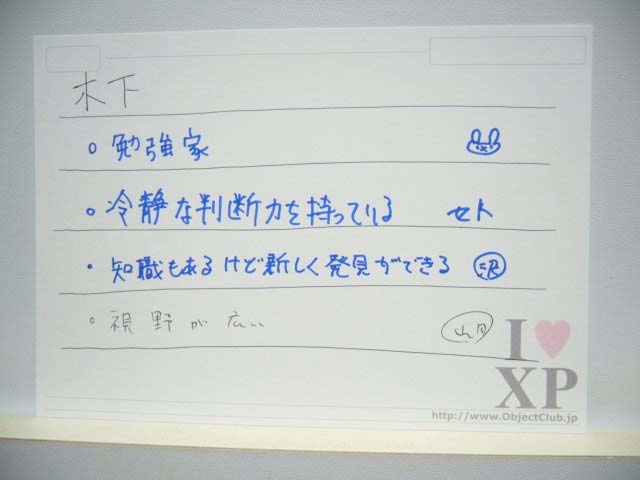
\includegraphics[width=\textwidth]{figures/positive-strokes.png}
	\caption{Positive stroke card provided by Kinoshita ~\cite{Kinoshita2008}}
	\label{figure:positive-strokes}
\end{figure}

\subsubsection{Timelines}
Derby et al. ~\cite{Derby2007} describes a process for a timeline activity, where the time spent is from thirty to ninety minutes. During the actual activity the retrospective leader should encourage all participants to engange in the discussion, with the goal of seeing the project from many perspective. The participants of the retrospective should be divided into multiple groups, where every member gets markers, and post it notes. The participants should then write their own issues during the project. These should be written down on color coded post its, where the color relates to a feeling or emotional state. Alternatively  the colors can represent events, functions or themes. When the groups are done filling out their post its, place them on the timeline. Let all the participants look at the created timeline, before taking a break or lunch. After the break the group should analyze the timeline, looking for interesting patterns that can be used for future improvements.

\begin{figure}[h!]
	\centering
	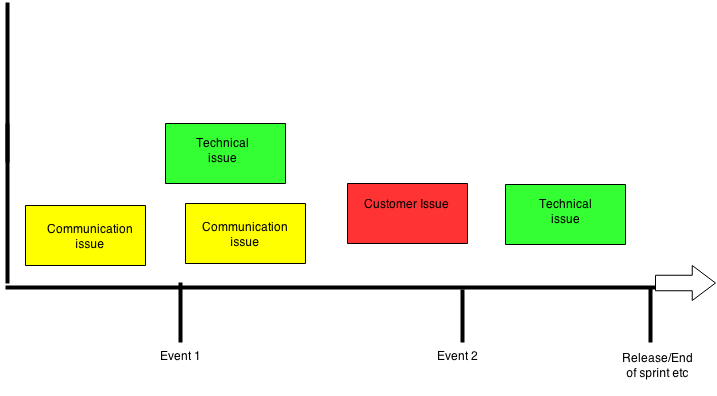
\includegraphics[width=\textwidth]{figures/Timeline-Example.png}
	\caption{A very simple timeline showing a set of different issues over time, where the issues are color coded}
	\label{figure:Timeline-Example}
\end{figure}

\subsubsection{Evidence based Timelines}
In an agile retrospective the Timeline exercise is an exercise aimed at supporting the evaluation of the issues and changes within a project. Bjarnson and Regnell~\cite{Bjarnason2012} describes how timelines should be based on evidence, and that this evidence should be time-stamped data that is collected through available systems in the environment of the project. The need need for evidence is because the memory of a participant can be biased or incorrect. In preperation for the timeline activity the timeline should be sent out to the participants of the retrospective, along with a set of reports that will be discussed during the actual retrospective. As the retrospective begins the history of the project is visualized, typically by posting the timeline created on a wall or blackboard, this timeline usually goes from the start of the project, to the end. The timeline could also be tailored to just contain a sprint, iteration or release within the project. As issues and events are placed on the timeline they are discussed by the participants of the retrospective. The participants themself should correct incorrect events, as well as add their own if needed. As the timeline is corrected and clarification added the meeting produces a timeline of events and issues that the relevant participants agree upon. The patterns and tendencies that emerege from the project timeline are then considered and evaluated in order to facilitate potential improvements. As multiple timelines are produced using the same template, over time this makes comparision analysis simpler. 

\begin{figure}[ht!]
	\centering
	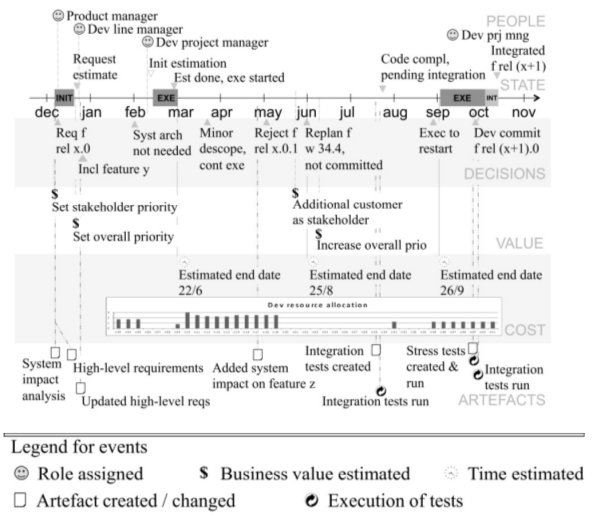
\includegraphics[width=\textwidth]{figures/timeline-derby.png}
	\caption{An example of an evidence based timeline as presented by Bjarnson and Regnells~\cite{Bjarnason2012}}
	\label{figure:Timeline-Derby}
\end{figure}

\subsubsection{Fishbone diagram - Ishikawa diagram}
One of the cause analysis methods used is the Ishikawa diagram, commonly known as fishbone diagram. Dingsøyr~\cite{Dingsoyr2005} describes the process of fishbone diagrams as follows:
\begin{quote} The process leader draws an arrow on a whiteboard indicating the issue being discussed, and attach other arrows to this one like in a fishbone with issues the participants think are causing the first issue. Sometimes, also underlying reasons for some of the main causes are attached as well.
\end{quote}
In \autoref{figure:fishbone-example} we give an example on how the issue late for work could be represented through a fishbone diagram. 

\begin{figure}[h!]
	\centering
	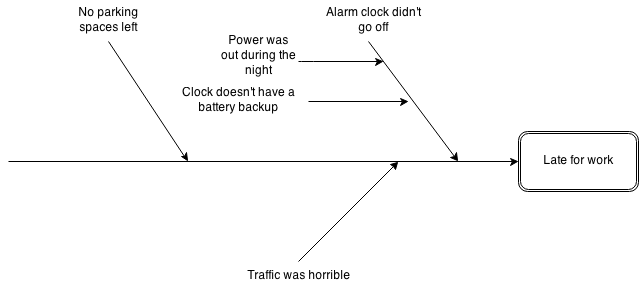
\includegraphics[width=\textwidth]{figures/fishbone-example.png}
	\caption{Fishbone diagram showing the cause analysis of the issue of arriving late for work.}
	\label{figure:fishbone-example}
\end{figure}

\subsubsection{Causal Map Analysis}
Bjørnson, Wang and Arisholm~\cite{Wang2012} proposes an alternative to fishbone diagrams in the form of causal map analysis. This is conducted in a similar way to the KJ-sessions, described above. The participants are given post-it notes on which they separately write down the causes of the issue the group is analyzing. They each then present their causes for the rest. When all causes are up on the whiteboard the participants together group the causes were able before they draw cause-effects relationships between the causes indicated by arrows. The group then are allowed to write new notes finding deeper or missing causes and place them in the map. This process continues until the participants are satisfied with the analysis. \autoref{figure:causalmap-example} gives an example of a causal map identifying the causes of the issue of arriving late for work.

\begin{figure}[h!]
	\centering
	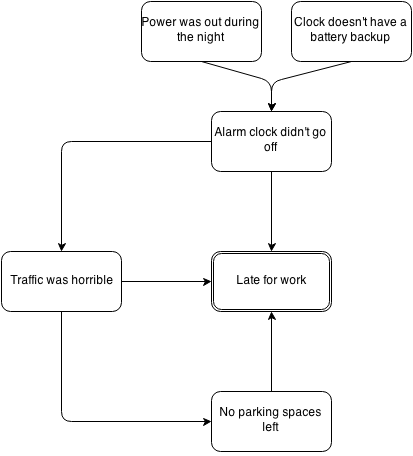
\includegraphics[width=0.7\textwidth]{figures/causalmap-example.png}
	\caption{Causal map showing the cause analysis of the issue of arriving late for work.}
	\label{figure:causalmap-example}
\end{figure}

\subsection{Other Findings} 
So far we have showed what practices and techniques could be employed during an agile retrospective and compared these against one another. However we also came across some other findings related to what to do during the retrospective, but not any specific practice or techniques. These findings will be presented in the following sections. 

\subsubsection{Discussion on Decision Making}
M. Drury, K. Conboy and K. Power ~\cite{Drury2012} did a focus group study on obstacles to decision making in agile development and found that one obstacle was uncertainty on who was responsible for acting upon decision made. They make the conclusion that as a part of the retrospective one should do a discussion on decision making. The reasoning behind this are that the retrospective is the only opportunity to evaluate the short-term tactical decision in relation to the bigger long-term strategic ones. They also predicts that doing discussion on decision making during a retrospective will help follow up upon the decision made. By clarifying owners for acting on decision made one removes the uncertainty on who is supposed to act on it, and thus the decisions will not be forgotten. 

\subsubsection{Globally dispersed teams holding retrospectives}
The rise of globally dispersed teams has led to challenges in holding retrospectives. The first major challenge is actually arranging a face to face meeting, due to the large geographical distances. This leads to potentially high travel cost both in time spent traveling as well as transportation cost. An option is to hold a virtual retrospective instead of face to face meetings. Holding virtual retrospectives is discussed by Terzakis~\cite{Terzakis2011} in his article. Terzakis describes the process of holding a virtual retrospectives, and the challenges needed to be overcome. A major challenge in very dispersed team is dealing with time zones. In the example in the article the teams are 10 hours apart, resulting in careful planning in order to make the impact on the team members as low as possible. Another challenge is to overcome differences in language and culture, this can be helped by agreeing on a glossary of terms as well as recognizing cultural differences. The exercise in the example is the timeline exercise, and it is completed with the help of digital tools. The tools used is a combination of email, spreadsheets and an audio bridge. Due to the usually highly interactive nature of retrospectives the tools chosen should be chosen carefully in order to engage all participants. The facilitator gains a lot of extra responsibility in planning the retrospective and understanding the potential variations between teams. Extra facilitator training might be necessary in some cases. The main challenges in holding a virtual retrospective is seen in the following table.

\begin{table}[!h]
	\centering
	\captionsetup{justification=centering}
	\caption{Issues in virtual retrospectives}
	\label{table:issues_virtual}
	\begin{tabular}{| l | p{0.3\textwidth}|}
	\hline
	Issue & Example of issues \\ \hline
	Logistics & Time zones differences, choosing tools \\
	Cultural differences & Importance of family, social norms difficulty speaking English (or another common language) \\
	Safety & Openness between team members \\
	Fairness & Some teams might dominate the discussion \\
	\hline
	\end{tabular}
\end{table}	





\subsubsection{Working Agreement}
M. Maham ~\cite{Maham2008} explains how to facilitate and conduct agile retrospectives. He suggest that starting with creating a working agreement so one can maintain a clear focus and get as much out of the time invested in the retrospective. 

\subsubsection{Put Improvement Actions in Backlog}
One of the main benefits of the agile retrospective is to be able to improve on ones processes by selecting improvements actions and work on those through the next phase of the development. M. Maham ~\cite{Maham2008} suggests to not only select the improvements actions, but put them in the backlog for the next development iteration. This would make the actions easy to track and remember through the next iteration. 

\section{After the Retrospective}
The final phase of the retrospective is after the retrospective meeting is conducted. Our study revealed three topics of things to consider after the retrospective meeting is finished. These topics are: Improvements follow-up and documentation. Our findings will be described below.

\subsection{Improvements Follow-up}
As one of the main benefits the retrospective allows one to improve on ones development practices. The retrospective meeting helps identify improvements and such one can create actions to implement these improvements. Creating the actions however does not by themselves implement the improvements one has to perform and follow-up upon them as well. This however can be a challenge. We only found two articles ~\cite{Drury2012, Collier1996}, mentioning this topic. They identified several obstacles that hindered follow up and some concrete actions to increase organizational knowledge. 

One of the obstacles identified was uncertainty of who was responsible to act on the decision made at the retrospective. One of the case studies under observation revealed that issues were never addressed and improvements never came, thus issues repeated over several retrospectives. This can be hazardous and teams may lose their will to perform retrospective, only seeing them as a waste of time. 

Another obstacle identified was that tactical decisions took priority over strategic ones. Tactical decisions, things to meet short term goals, was considered by agile teams to me more demanding and important than strategic ones. This resulted in the people responsible for follow-up upon the actions from the retrospective rather would consider daily tactical tasks rather than the strategic ones from the retrospective. This again can result in improvements never occur and people losing the will to perform retrospectives. 

Collier et al. Suggests four actions which would increase the organizational knowledge. The first action should be storing all the outputs from the retrospective. The second action recommended is to categorize all lessons learned by their functional area. Then assign each item to a specific person for the next project and make him report back to leadership on its progress. The third action is for one of the team members to present the results from the postmortem for the upper management at their regularly organizational reviews. The final action recommended by Collier et al. is to assign each lesson learned to a person in the organization who will be held responsible for investigating and implementing a solution. 

\subsection{Documentation}
After the retrospective several articles ~\cite{Dingsoyr2005, Moe2001, Hanssen2003, Collier1996} suggests writing a report from the retrospective meeting. \todo{TODO: is there different advice in the literature depending on the development method used?}

Dingsoyr~\cite{Dingsoyr2005} elaborates that if one of the goals of the retrospective is to transfer knowledge to people outside the project one should write a report that explains what went well, what went wrong, the causes and what was said during the meeting. If the intention is to only find improvement actions these should be documented. \todo{TODO: Write about whether in big company or in small company}

Collier et al.~\cite{Collier1996} recommends another format for the documentation of the report. First the report should contain a brief project description including the unique aspects of the project. The next should be a summary of the positive findings of the postmortem. Then a summary of the three worst factors that hindered the team from reaching their goals. And finally the report should include one improvement action, describing the problem and the actions to counter it. 

\section{Enthusiasm for the Agile Retrospective}
The second main view of our literature review is about enthusiasm. Throughout most of the articles we read the responses from participants was mentioned, if only briefly. 

In a case study~\cite{Hanssen2003} assessing the retrospective using KJ-sessions and Fishbone diagrams feedback from the participants was given. They believed that it was useful, and it was easy to grasp so everybody could participate. They also said they felt like the got something back for participating. New insights and ways to improve their job were some examples given by the researchers. 

In a controlled experiment performed by Bjørnson, Wang and Arisholm ~\cite{Bjornson2009} on students performing postmortem reviews, the researchers got feedback on the impression of the methods used. All the students participating responded with positive impressions regardless if they performed fishbone diagram or root cause analysis. The authors did however observe that the enthusiasm was lower when performing cause analysis than when doing KJ-sessions. This seems to fit well with the ``lesson learned'' by Stålhane et al. ~\cite{Hanssen2003}  that some developers did not participate much in the root cause analysis. 

However not all are satisfied with the retrospectives. Drury et al. ~\cite{Drury2012} reflects on their findings: 
\begin{quote}
To some, the Iteration Retrospective appears a waste of time because people just talk about issues but no one takes them on board to make changes in the process in future iterations.
\end{quote}
This shows that even though many are happy with performing retrospectives there are some that just sees it as a waste of time. 

\clearpage

\part{Discussion}
Using a ``grounded approach'' inspired process we identified several views on the agile retrospective. We will now discuss our results and provide an overview over the research domain of agile retrospectives.

\section{Retrospective Practices}
\subsection{Planning the retrospective}
The first thing we want do discuss is the planning of a retrospective. Dingsøyr~\cite{Dingsoyr2005} presented several steps to planning a retrospective. They included deciding to hold a retrospective, declaring the intent, find the participants and selecting the exercises, before collecting objective data on the project. We believe that this is a healthy process of conducting a retrospective. A retrospective should not be held solely on the reason of holding a retrospective. 

\subsubsection{Wish to Improve} 
To achieve the most out of a retrospective one should first have a wish to improve some aspect of ones development process, thus deciding to hold a retrospective meeting. 

\subsubsection{Declaring a Goal}
When one has decided to hold a retrospective one should further plan the intent of the retrospective. You cannot plan without a goal, and without a plan most things tend to not reach their full potential. We believe retrospectives are no exclusion to this. The fact that several articles~\cite{Dingsoyr2005, Bjornson2009, Hanssen2003, Maham2008, Birk2002, Moe2001} describes concrete planning steps or suggest using external facilitators seems to fit well that one should plan for the retrospective. 

\subsubsection{Participants}
Who to include in the retrospective meeting provides multiple concerns to consider. The current literature differentiates between four types of participants: Team member, managers, customer and external facilitator. The four types have different roles in the retrospective and should be included based on what the goal of the retrospective should be. 

The team member takes part as a participant contributing knowledge and insight during the meeting. According to Dingsøyr ~\cite{Dingsoyr2005} one want to include as many as possible to get different kinds input. Team members should always participate during retrospective.

Managers can take part as either a participant contributing knowledge or as an internal facilitator leading the meeting. However it is not recommended by Dingsøyr ~\cite{Dingsoyr2005} to include managers as the other team members can be intimidated to not honestly share issues as the manager is also the one evaluating them. If one want as much knowledge as possible one should not include managers during retrospective meetings.

The customer can participate as a knowledge contributor during retrospectives. It is however not recommended ~\cite{Dingsoyr2005} to include the customer as the focus then can change from process improvement to customer relations. If the goal however is to improve customer relations we assume bringing the customer along would be a good idea, even though we haven't found any studies bringing up the subject. But in any other case the customer shouldn't participate.

The external facilitator participates in a facilitating role. Through encouraging discussion, leading activities and providing a fresh set of eyes the facilitator can improve retrospectives by providing neutral ground and provide new angles to look at problems. If available one should include an external facilitator to improve the value of the retrospective.

The four types of participants in a retrospective provides an overview of whom one should include as can be seen in \autoref{table:participants}. It is recommended to include as many team members as possible and use an external facilitator. It is however not recommended to include either managers or customers into the meetings, as this can hinder an open arena for discussion. 

\begin{table}[!h]
	\centering
	\captionsetup{justification=centering}
	\caption{Participants, their roles and whether they should be included in a retrospective meeting.}
	\label{table:participants}
	\begin{tabular}{llp{0.3\textwidth}}
		\hline
		Participant Type: & Role: & Should Participate?\\ \hline
		Team member & Knowledge contributer & Yes, as many as possible. \\
		Manager & Knowledge contributer & No, can hinder open discussion \\
		& Facilitator & \\ 
		Customer & Knowledge contributer & No, changes focus from process improvement to customer relations \\
		External facilitator & Facilitator & Yes, if possible \\ 
		\hline
	\end{tabular}
\end{table}


\subsubsection{Preparing the Retrospective} \label{subsec:which-techniques}
When all goal is set, participants decided and objective data collected one need to decide which techniques one should use during the actual meeting. The results of our literature review revealed several techniques to use. The choice of which technique to use should reflect the goal one has set for the retrospective. We have through our analytical approach grouped the different techniques listed in \autoref{subsec:technqiues-identified} into four types of goals that represents the process. These goals are ``Identify issues'', ``Improve estimations'', ``Feedback'' and ``Problem understanding''. We will elaborate on these goals and the techniques defined within them in the following sections. In \autoref{table:technique-discussion} we have provided an overview of the different techniques, with their goals, costs and outputs attached. 

\paragraph{Identify Issues}
By identifying issues we mean that the technique helps discover issues currently present in within a development process. This issues can both be positive and negative. The techniques that we've categorized to have the goal of identifying issues are: KJ-sessions, Keep Problem Try (KPT), Timelines and Evidence based Timelines. Each of the four techniques provide a way of identifying issues by different means. 

The three techniques: KJ-session, KPT and Timelines, lets the participants identify the issues occurring in a current project. This is done by letting the participants writing down their own issues and presenting them to the group. The thing that differs between this three techniques is how they issues are grouped after being identified. In KJ-session the issues are grouped by means of whether they are related to each other resulting in issue groups that can be analyzed. In KPT the issues are grouped by whether they are positive or negative. Positive issues are grouped as Keep while negative is grouped as Problem. Using these one performs an informal analysis that results in improvement actions, grouped as Try. In Timeline the issues are placed in the order of where they occur  chronologically in the timeline. This can help identify interesting patterns that can be analyzed. These three techniques we identify as low cost as no to little preparation is needed and one can perform the practice quickly if wanted. 

The fourth issue identifying technique is evidence based timelines. This technique differs from the others as it require the facilitator to present the issues for the participants. This is done by the facilitator placing issues along a time line based upon hard data acquired through the project/iteration. For each issue presented by the facilitator a short discussion commence to assure that all agrees. If some issues are wrong or some issues are missing the participants are required to provide corrections to the issues or add the issues. When the timeline is complete it can help identify interesting patterns that can be analyzed in similar way to the timeline technique described above. As this practice require a substantial amount of preparation from the facilitator, but they same amount of time as the techniques described above, we classify this as medium cost process.

Through our literature review we did not find any comparisons between these four method of identifying issues, neither empirical or experience based. Studies reveals only the feedback received while using one of the methods. Interestingly all techniques have positive feedback, which in turn leaves us to believe that regardless of which technique one uses it will give some valid output. This implicates that one can choose which technique oneself prefers.

\paragraph{Improve Estimation}

\begin{table}[!ht]
	\centering
	\captionsetup{justification=centering}
	\caption{An overview table of different retrospective techniques}
	\label{table:technique-discussion}
	\makebox[\textwidth]{%
	\begin{tabular}{p{0.3\textwidth}p{0.35\textwidth}p{0.1\textwidth}p{0.35\textwidth}}
	\hline
	Technique & Goal & Cost & Output \\ \hline
	KJ-Sessions & Identify issues & Low & A set of grouped issues \\ 
	Keep, Problem, Try & Identify issues & Low & Set of positive issues \\
	& & & Set of negative issues \\
	& & & Set of improvement actions. \\ 
	Estimation Retrospective & Improve estimations & Low & Insights for estimations \\ 
	Experience Reports & Problem understanding &  Low & Experience related to contract issues, design and technology \\
	Positive strokes & Feedback & Low & Individual feedback to each team member \\
	Timelines & Identify issues & Low & Chronological outline of issues \\ 
	& Problem understanding & & Improvement actions \\
	Evidence based timelines & Evidence based issue identification & Medium & Chronological outline of evidence based issues \\
	& Problem understanding & & Improvement actions \\
	Fishbone & Problem understanding & Low & Issue analysis \\
	& & & Improvements actions \\
	Causal map analysis & Problem understanding & Low & Issue analysis \\
	& & & Improvements actions \\
	\hline
	\end{tabular}
	}
\end{table}


\subsubsection{Collect Data}
After determining the goal, decided on techniques and invited the participants, data has to be prepared for the meeting. This data can be related to the project in general, needed for techniques or collected through surveys to prepare the facilitator for leading the retrospective meeting. Regardless of what the data is in relation to it has to include both positive aspects and negative aspects. This according to Stålhane et al. ~\cite{Birk2002} will help avoid forgetting working practices. 

Several methods are described for collection the objective data before the retrospective. Survey is an efficient, quick and low cost process for obtaining data according to Collier et al. ~\cite{Collier1996}. It helps establishing the scope for the retrospective and severity of different issues. It also returns quantitative data for organizational use.

Interviewing is another method described by Stålhane et al. ~\cite{Birk2002}. It is a powerful way of gathering information, and set this information in a personal context that can be beneficial in cases where personal feelings have to be included. It is however more costly as it requires more time from both facilitator and participants. 

The last method mentioned by Collier et al. ~\cite{Collier1996} is collecting objective information. Objective information is valuable for the retrospective for four reasons according to Collier et al. It will help identify the biggest improvement opportunities. It gives easier comparison between different projects. It gives feedback on scheduling efforts. And it helps focusing discussions. 

By using various techniques one can collect data to help prepare and improve the retrospective. In \autoref{table:data-collection} we provide an overview over the techniques described above. 

\begin{table}[!ht]
	\centering
	\captionsetup{justification=centering}
	\caption{Techniques for collecting data before a retrospective}
	\label{table:data-collection}
	\makebox[\textwidth]{%
		\begin{tabular}{ l  l  p{0.6\textwidth} }
			\hline
			Technique & Cost & Main Benefit \\ \hline
			Survey & Low & Helps establish scope of retrospective as well as severity of issues. \\
			Interviews & High & Obtains data in a personal context \\
			Objective Data Collection & Low & Will help identify larger improvement opportunities. Helps focusing discussions. \\
			\hline
		\end{tabular}
	}
\end{table}

\subsection{During the Retrospective}
During a retrospective meeting there are several issues to be aware of. As a facilitator maintaining an open arena for discussion can be difficult. Remembering to assign decision owners for improvement actions can be easy to forget. We will discuss these practices in the following sections. We have also provided a table over possible pitfalls and considerations to remember in \todo{TODO: CREATE THIS TABLE}

\subsubsection{Openness}
A. Birk, T. Dingsøyr and T. Stålhane ~\cite{Birk2002} suggests that while performing a retrospective one shouldn't limit experience gathering to the project's negative aspects. One should also identify the positive aspects as well or they might go unnoticed. 
\todo{Every view should be presented.}

\todo{Remember both positive and negative views.}

\subsubsection{Assign Decision Owners} \label{par:assign-decision-owners}

\subsection{After the Retrospective}
Even though the retrospective meeting is completed the work aren't completely over. 

\subsubsection{Follow up}
Through the retrospective meeting one has identified different issues and actions to resolve these. Until the next retrospective the job of resolving these issues has to be done. 

Through our literature review we found only one clearly defined action to help improve resolving identified issues. The one action clearly defined was to assign owners to the improvement actions. By doing this several articles ~\cite{Collier1996,Drury2012} assumes that it will help resolve these issues, as when an owner of an issue is held responsible for issue being worked on. If no owner would be assigned other tasks would get prioritized. Thus the issue would never be resolved. By declaring an owner for an action resolving an issue, it is assumed it will be resolved. However we have not seen any research been done in this part of agile development and we believe the lack of defined actions may be the cause for issues recurring throughout several retrospectives. 

\subsubsection{Documentation}
The second activity that are due after the retrospective is documenting it. Different research suggests different kinds of documentation. Some suggests ~\cite{Collier1996} writing lightweight reports containing project description, positive issues, negative issues and actions to resolve the negative ones. 

Dingsøyr~\cite{Dingsoyr2005} recommends considering the size of the company as well as the distribution of the report. If the company is big then one should use time to codify the knowledge, but if the company is small one could do with only write a short report as the knowledge will be spread anyways. 

\section{Enthusiasm}

\paragraph{Positive to Practices}

\paragraph{Recurring Issues Kills the Joy}

\todo{not the how you do it, but the value of it}

\section{Conclusion}
Throughout this article we have evaluated agile retrospective practices and found their weaknesses and strengths based on existing literature. Our findings revealed that practices today provides a big variety of techniques each fitting for different kinds of goals. \todo{TODO: Include something about enthusiasm.} We do however believe there is a gap in current research considering the follow-up of issues identified in agile retrospectives. There seem to be few clearly defined processes/actions that handles this area. And we believe that this may be a reason for the falling enthusiasm of the retrospective. 

Our contribution has been to create an overview of the existing literature on the research on agile retrospectives, where we have evaluated the strengths and weaknesses of practices and identified a possible gap in current literature. \todo{TODO: add something about practitioners!}

\clearpage

\bibliography{references}
\bibliographystyle{plain}
\end{document}